\begin{frame}{\og{}Napoléon des névroses\fg{} ou \og{}Paganini de l'hystérie\fg{} {\small(\hypersetup{citecolor=yellow}\cite{marmion2015freud})}}

\textsc{\textcolor{deepblue}{\textbf{Jean-Martin CHARCOT}} (1825-1893)} 
%\hbox{\hspace{25em} 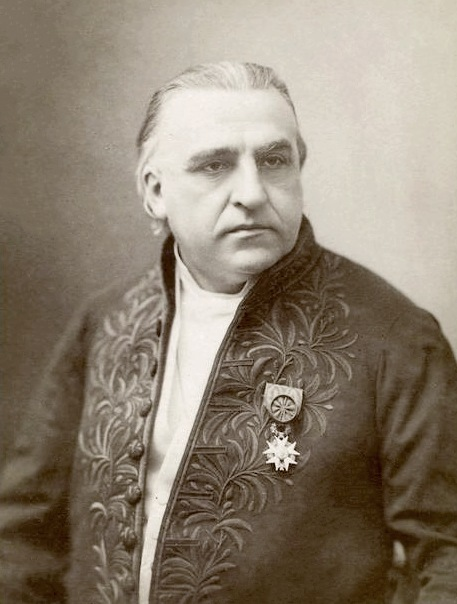
\includegraphics[scale=0.07]{pic/Jean-Martin_Charcot.jpg}}
%\\{\scriptsize Portrait de\\Charcot (\href{https://fr.wikipedia.org/wiki/Jean-Martin_Charcot}{Wikipedia}).}
\hbox{\hspace{10.3em} 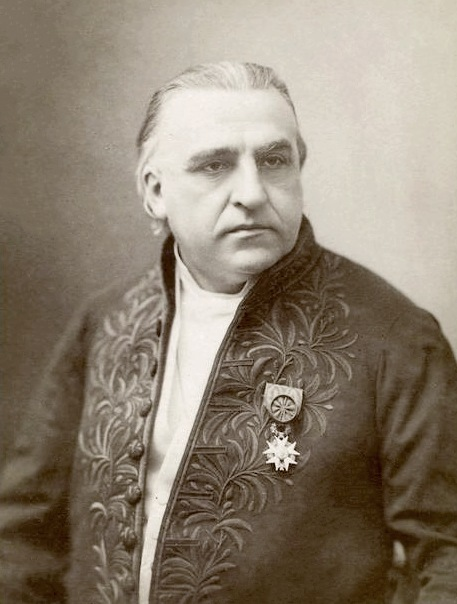
\includegraphics[scale=0.06]{pic/Jean-Martin_Charcot.jpg}}\\\hbox{\hspace{23.8em}{\tiny Source : \href{https://fr.wikipedia.org/wiki/Jean-Martin_Charcot}{Wikipedia}}.} \pause
\begin{itemize}[<+->]
\item père de la neurologie moderne en France au XIX\ieme{} s. 
\item leçons cliniques du mardi à l'hôpital de la Salpêtrière à Paris \\
\hspace{165pt}
\footnotesize\og{}Mecque de la neurologie\fg{}
\end{itemize}

\begin{enumerate}[\indent {}]
\only<4->{\item Contributions majeures:}
\small
    \begin{tabular}{l l}
    \only<5->{\textcolor{darkgray}{hystérie} & $\leftarrow$ lésion dynamique des circuits cérébraux} \\
    \only<6->{\textcolor{darkgray}{hypnose} & analyse et traitement des symptômes hystériques} \\
    \only<7->{\textcolor{darkgray}{SEP} & description de la \textit{sclérose en plaques} disséminée} \\
    \only<8->{\textcolor{darkgray}{SLA} & description de la \textit{sclérose latérale amyotrophique}} \\
    \only<9->{\textcolor{darkgray}{maladie de Parkinson} & concepteur du terme (avec A. Vulpian)} \\
    \end{tabular}
\end{enumerate}
%\begin{itemize}[<+->]
%\small
%\item[] \textcolor{darkgray}{hystérie} & $\leftarrow$ lésion dynamique des circuits cérébraux 
%\item[] \textcolor{darkgray}{hypnose} & analyse et traitement des symptômes hystériques 
%\item[] \textcolor{darkgray}{SEP} & description de la \textit{sclérose en plaques} disséminée 
%\item[] \textcolor{darkgray}{SLA} & description de la \textit{sclérose latérale amyotrophique} 
%\item[] \textcolor{darkgray}{maladie de Parkinson} & concepteur du terme (avec A. Vulpian) 
%\end{itemize}
\pause
%\vspace{-0.3cm} \pause
\begin{flushright}
{\footnotesize(\cite{camargo2024jean})}
\end{flushright}

%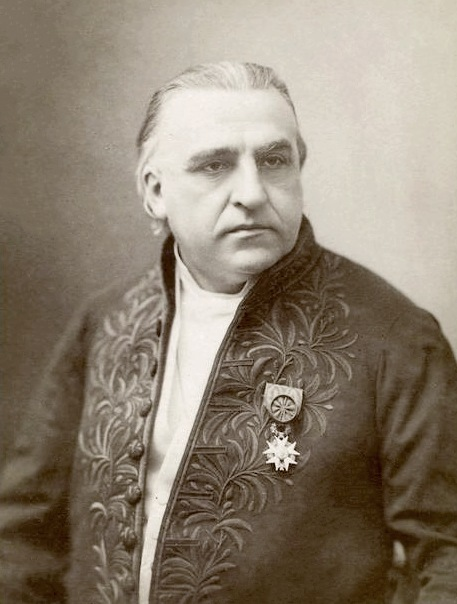
\includegraphics[width=10pt]{pic/Jean-Martin_Charcot.jpg}%
%\\{\scriptsize Portrait de\\Charcot (\href{https://fr.wikipedia.org/wiki/Jean-Martin_Charcot}{Wikipedia}).}



\end{frame}
\begin{frame}{Impact de Charcot sur sa discipline et au-delà}
\centering
\textbf{Collaborateurs et élèves} \pause \\
{\small \og{}réseau scientifique\fg{}} \pause
    \begin{table}[!ht]
        \centering
        \small
        \begin{tabular}{l l r}
           \only<3->{Sigmund \textsc{Freud} & 1856-1939  & théorie psychanalytique} \pause \\
            \only<4->{Gilles \textsc{de la Tourette} & 1857-1932 & syndrôme de Tourette} \pause \\
            \only<5->{Joseph \textsc{Babinski} & 1857-1904 & pithiatisme, signe de Babinski} 
%           Pierre \textsc{Janet} (1859-1947) & psychopathologie
%            dissociation, sous-conscient 
        \end{tabular}
        \pause
        \begin{flushright}
%        \footnotesize\citep{bogousslavsky2020}
        \footnotesize\citep{BROUSSOLLE2012301}
        \end{flushright}
        % \caption{Caption}
        \label{tab:my_label}
    \end{table}
    \pause
\medskip
\textbf{Écrivains naturalistes français et européens} \pause
\begin{itemize}
\centering
\small \item références à Charcot et aux descriptions de crises hystériques
\end{itemize} \pause
\begin{table}[!ht]
    \centering
    \small
    \begin{tabular}{l l r}
        \only<9->{Émile \textsc{Zola} & 1840–1902  & \textit{Lourdes}} \\
        \only<10->{Léon \textsc{Tolstoï} & 1828–1910 & \textit{La Sonate à Kreutzer}} \\
        \only<11->{Luigi \textsc{Capuana} & 1839–1915 & \textit{La Torture}}
%        Bjørnstjerne \textsc{Bjørnson} (1832–1910) & \textit{Over Ævne}
    \end{tabular}
    \pause
    \begin{flushright}
    \footnotesize\citep{koehler2013charcot}
    \end{flushright}
    % \caption{Caption}
    \label{tab:my_label}
\end{table}

\end{frame}

\begin{frame}{Question de recherche}
% Comment mesurer le degré d'intertextualité entre Charcot et son réseau scientifique et artistique au prisme du numérique ?
% create the main block
\begin{exampleblock}{}
\centering
    \color{deepblue}{\textmd{Comment mesurer le degré d'intertextualité entre Charcot et son réseau scientifique au prisme du numérique ?}}
\end{exampleblock}

\end{frame}
